\documentclass[a4paper]{article}

\usepackage[utf8]{inputenc}

\usepackage{url}
\usepackage[]{hyperref}

\usepackage{caption}

\usepackage{listings}

\usepackage{color}

% *** GRAPHICS RELATED PACKAGES ***
%\usepackage[pdftex]{graphicx}
\usepackage{graphicx}
%\usepackage[dvips]{graphicx}
% to place figures on a fixed position
\usepackage{float}

\usepackage{amsmath}

\usepackage[margin=1in]{geometry}

\title{Inspecting High-speed transport protocol simulations}
\author{Sonkoly, Balázs (transzport protocols); Németh,Felicián (Network Simulator);Császár András (Network Simulator) }
\date{}


\begin{document}

\maketitle

\tableofcontents

\section{Introduction}

\textbf{Transmission Control Protocol (TCP)} has been used for congestion control in the Internet for decades. During the evolution of the Internet a lot have been changed about the traffic patterns of applications and also in the structure of the networks. Wireless and high-speed network environments pose new challenges that can be tackled by current TCP version only at the price of many trade-offs.

TCP -- one of the most important transport protocol of the Internet -- has a history of many decades. The initial protocol -- that was called \emph{Network Control Protocol - NCP} -- is originated from the '70s. Out of this protocol had emerged the TCP/IP network's two foundational protocols: IP operating in the network level, and TCP~\cite{CongestionAvoidance} operating in the transport level. TCP has many features that are required for proving reliable transport services. Congestion control is one of its main feature that protects the network from over-utilization. The connection-oriented TCP protocol does closed-loop control during which the transmitter adjusts its transmission speed based on the incoming acknowledgments affected by the network conditions aimed for having optimal network utilization and to avoid network breakdown by over-utilization. The initial version was finalized in \href{http://www.faqs.org/rfcs/rfc793.html}{RFC 793} in 1981. The base mechanism had been extended gradually with new methods like \textbf{Slow Start}, \textbf{Congestion Avoidance}, RTO calculation, delayed acknowledgment in 1989(\href{http://www.faqs.org/rfcs/rfc1122.html}{RFC 1122}), selective acknowledgment (\textbf{SACK}) in 1996 (\href{http://www.faqs.org/rfcs/rfc2018.html}{RFC 2018}) or definition of \textbf{NewReno} version in 2004 (\href{http://www.faqs.org/rfcs/rfc3782.html}{RFC 3782}).

\section{Conventional TCP: TCP Reno}

TCP's main task is implement congestion control in a distributed, closed-loop system in a way that the users can utilize the available network bandwidth in an optimal and fair manner. The latter attribute is commonly referred as a protocol's \textbf{fairness} that is going to be a main aspect in future network's beside efficiency. In case of new protocols and new control mechanisms -- in contrast with traditional TCP's traditional design methodology -- the findings and theory of control theory and optimization theory can be utilized during the design phase.

During a TCP connection the transmitting party sends data packets over the network and the receiving side provides cumulative acknowledgments that informs the sending side about the so far correctly received packets. The TCP transmitter can send a new packet in case of a received acknowledgment that realizes a from of closed-loop control (\textbf{self-clocking}). In TCP the congestion control is realized using a sliding-window mechanism where the transmitter can only have a number of outstanding unacknowledged packets in the network corresponding to the size of the \textbf{congestion window (cwnd)}. The size of the congestion window is a state variable (beside many others) controlled by the transmitter entity that can be used for controlling the transmission speed. The main task of the congestion control algorithm is to control this state variable as a function of the network conditions. TCP Reno controls this \emph{cwnd} variable differently in different phases of the connection. After connection establishment -- when the network conditions are yet unknown on the network path -- the control of the cwnd and the speed happens using the \textbf{Slow Start} algorithm. In this phase -- despite the name of the algorithm -- the congestion window expands exponentially until it reaches a threshold or packet loss occurs. After one of these events the long term behavior is determined by the \textbf{Congestion Avoidance} phase when the protocol tries to control the transmission speed so that it won't cause severe congestion in the network. In this phase the congestion window is controlled by the \textbf{AIMD} (Additive Increase Multiplicative Decrease) mechanism. As a result of this control the congestion window takes on a typical oscillating, sawtooth pattern.

There are two more mechanisms worth noting here that performs correction of lost packets. These are the \textbf{Fast Retransmit} and \textbf{Fast Recovery}. When TCP reno detects multiple ACKs for the same packet (that means the receiver still expects to receive the same packet) then it implies a packet loss event with not significant congestion since the subsequent packets have reached the receiver successfully. After 3 duplicate ACKs it retransmits immediately the missing packet (Fast Retransmit) and transfers into Fast Recovery phase. The transmission does not cease in Fast Recovery phase, the transmitter can send new packets into the network based on the current value of cwnd and the received ACKs. As soon as the missing packet has been ACK-ed TCP Reno goes back into Congestion Avoidance. The protocol differentiates the packet loss due to extreme congestion using a timer that is started after sending each packet. If this timer expires (RTO, Retransmission Time Out) that means ACKs from the receivers are completely missing or too many packets have been lost. In such case TCP Reno implies extreme network congestion and restarts in Slow Start. The different phases of TCP Reno are illustrated on Figure~\ref{fig:TCP-Reno-operation}. Further details can be found in~\cite{CongestionAvoidance} (can be downloaded from \href{http://qosip.tmit.bme.hu/cgi-bin/twiki/viewfile/VITT5318/WebHome?rev=1;filename=jacobson88congestion.pdf}{here}).


\begin{figure}[H]
    \centering
    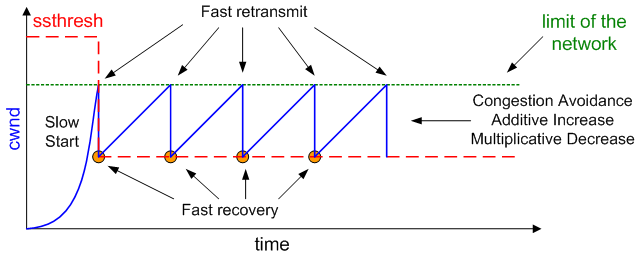
\includegraphics[width=0.9\textwidth]{figures/tcp-reno.png}
    \caption{The operation and phases of TCP Reno}
    \label{fig:TCP-Reno-operation}
\end{figure}

The properties of AIMD algorithm ensures that the TCP Reno flows transmission speed converges to the fair state in case of the flows have identical round trip time (RTT). This operation is illustrated by Figure~\ref{fig:AIMD}. Out of the linear control methods AIMD is capable to provide the convergence to the optimal state from any point in this state space for providing maximum utilization and fairness. Think about why not MIMD, AIAD and MIAD mechanism are not convergent!

\begin{figure}[H]
    \centering
    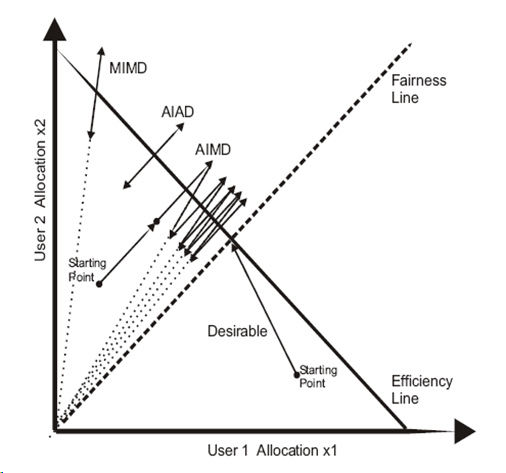
\includegraphics[width=0.9\textwidth]{figures/AIMD-trajectory.png}
    \caption{AIMD trajectory in case of two flows with equivalent RTT }
    \label{fig:AIMD}
\end{figure}

The sawtooth pattern originated from the AIMD can be examined on Figure~\ref{fig:sawtooth}. It's clearly visible that in case of no packet-loss the cwnd grows linearly (additive increase) and when a packet loss occurs the cwnd halves (multiplicative decrease). This operation is implemented by increasing cwnd by \textbf{cwnd} for each received ACK that roughly translates to increase by 1 under one RTT. In case of detecting a packet loss the cwnd is halved. The essence of the method in mathematical format is the following:

\begin{tabular}{ll} 
per-ACK: & $\texttt{cwnd} \leftarrow \texttt{cwnd} + \dfrac{1}{\texttt{cwnd}}$  \\
per-RTT: & $\texttt{cwnd} \leftarrow \texttt{cwnd} + 1$ \\
loss: & $\texttt{cwnd} \leftarrow \texttt{cwnd} - \dfrac{\texttt{cwnd}}{2}$ \\
\end{tabular}

\begin{figure}[H]
    \centering
    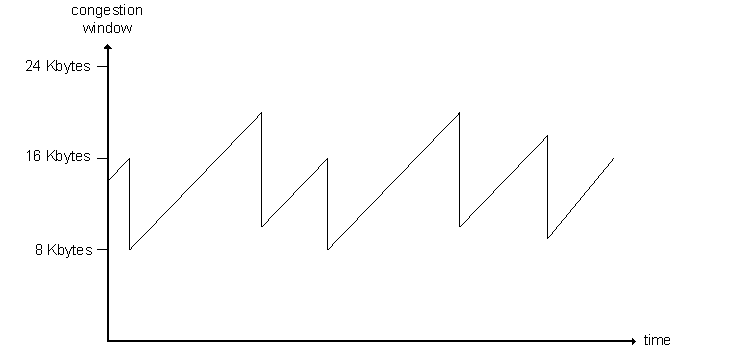
\includegraphics[width=0.9\textwidth]{figures/sawtooth.png}
    \caption{Sawtooth plot}
    \label{fig:sawtooth}
\end{figure}

The basic TCP reno mechanism is not efficient if multiple packets are lost under one round trip (packet loss burst) because this can not be corrected efficiently by the Fast Retransmit/Fast Recovery mechanism. For fixing this issue Selective Acknowledgment had been added (SACK) that can be used by the receiver to inform the transmitter in detail on which blocks of the packet sequence has been received and which are missing. This naturally involves modifying the implementation of both the sender and receiver TCP entity. Furthermore the TCP header is extended with a corresponding optional block (SACK option header). Nowadays most TCP implementations provide the SACK extension.


\section{Congestion control principles}

It has been shown that for TCP Reno the indicator for congestion is a packet loss event that occurs when the queues overflow on a link with the smallest bandwidth (i.e. the bottleneck link). This method -- called \textbf{packet loss based} congestion control -- is present in several new, high-speed TCP version however it has some drawbacks as well. The actual congestion control is can be carried in 1 bit of information (packet loss/no packet loss) as a consequence it does not allow fine-grained or sophisticated control algorithms to be used. Furthermore packet-loss based control involves filling up queues since the control action is only carried out in case of a packet loss. That infers the presence of oscillation that incurs  system wide stability issues. Another control approach is to measure the RTT of individual packets and control the transmission speed based on this input. These \textbf{delay-based} methods aims for a single TCP flow keeping a given amount of packets in the network queues along the network path. These protocols estimate the components of RTT using a certain method. The components are the physical propagation time and the queuing time. In these type of algorithms the latter one is subject to be controlled by different methods.
The newest methods combine the packet loss and delay-based methods into a \textbf{hybrid} algorithm for congestion control where the transmitter reacts to both packet loss and change in delay events. Even more sophisticated methods are applied by some protocols that utilize \textbf{passive or active measurement methods} for estimating the available network bandwidth and performing control. 

In the previously described methods the transmitter has the necessary logic  and the concrete algorithms can be improved flexibly or even replaced completely without changing other parts of the network. However there is a concept that the current state of the network congestion is reported by the network routers explicitly to the transmitter. These \textbf{explicit congestion signaling} methods requires modification of existing network routers.


\section{Further Reading}

\begin{itemize}
    \item \href{https://qosip.tmit.bme.hu/foswiki/pub/Meres/OpenFlowMScMeresiSegedlet/a19-lantz.pdf}{A Network in a
              Laptop: Rapid Prototyping for Software-Defined Networks}
    \item

          \href{https://qosip.tmit.bme.hu/foswiki/pub/Meres/OpenFlowMScMeresiSegedlet/mininet-hotnets2010-final.pdf}{Presentation
              of conference proceedings on Mininet}
    \item	Mininet page: \url{http://mininet.org/}
    \item	Mininet wiki: \url{https://github.com/mininet/mininet/wiki}
    \item	Mininet introduction: \url{https://github.com/mininet/mininet/wiki/  Introduction-to-Mininet}
    \item	Mininet Python API: \url{http://mininet.org/api/hierarchy.html}
\end{itemize}

OpenFlow specifications:
\begin{itemize}
    \item
          \href{https://qosip.tmit.bme.hu/foswiki/pub/Meres/OpenFlowMScMeresiSegedlet/openflow-spec-v1.0.0.pdf}{v1.0}
    \item
          \href{https://qosip.tmit.bme.hu/foswiki/pub/Meres/OpenFlowMScMeresiSegedlet/openflow-spec-v1.1.0.pdf}{v1.1}
    \item

          \href{https://qosip.tmit.bme.hu/foswiki/pub/Meres/OpenFlowMScMeresiSegedlet/openflow-switch-v1.3.4.pdf}{v1.3.4}
    \item

          \href{https://qosip.tmit.bme.hu/foswiki/pub/Meres/OpenFlowMScMeresiSegedlet/openflow-switch-v1.4.1.pdf}{v1.4.1}
    \item

          \href{https://qosip.tmit.bme.hu/foswiki/pub/Meres/OpenFlowMScMeresiSegedlet/openflow-switch-v1.5.1.pdf}{v1.5.1}

\end{itemize}

\appendix

\section{Entry quiz sample questions}

\begin{enumerate}
    \item Describe briefly the main concept of the OpenFlow recommendation.
    \item What are the components of an OpenFlow network?
\end{enumerate}

\section{Lab exercises}

\subsection{Lab environment}

\end{document}